% chap2.tex - Week 2
\chapter{Week 2}
\section{Day 1 - ``We are coders, we use Git!''}
\subsection{Setting Up the Environment}

So now we are ready to begin delving into and actually using Git, right? Well, not exactly.
First we have to decide upon how the workflow model we have envisaged is implemented in our version control system.
With Git being so versatile, it's both a blessing and a danger.
It is a good idea to define from early on, exactly how you would like the developers, lieutenants and dictators to behave, before you begin actually committing any code.
Sometimes this isn't possible.
It's quite feasible that you have never used a version control system like Git before and you begin by muddling your way through.
This is normal, but if you are in charge of implementing this type of system for a professional environment, you should really consider first how this is going to work.

Conceptually, the model which was discussed previously is easy to imagine.
We have two dictators, who both have access to the blessed repository and then several developers, who are going to have their changes reviewed and included, by the aforementioned dictators.
The physical representation of the workflow model is summarised in the diagram below.

\begin{figure}[bt]
\centering
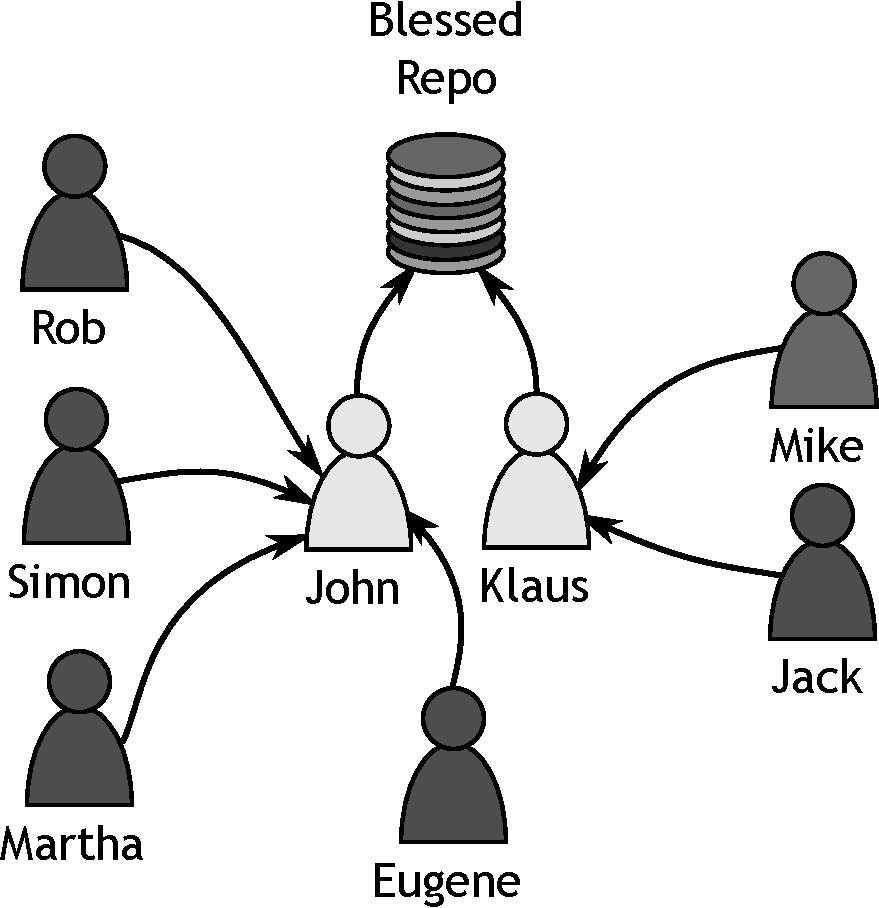
\includegraphics[width=7cm]{images/f-w2-d1.pdf}
\caption{Tamagoyaki Inc's Physical Structure}
\end{figure}

The physical structure is all well and good, but it doesn't determine exactly how the data is moved, just who is responsible for it at each stage in the process.
What is required, is a detailed analysis of where the data flows from and to.
A data flow diagram is useful, but not essential.
However, we will create a slightly different form of diagram to show how the data will be moved from one person to another.
Before we go ahead and look at the diagram, let's go back to the trenches to see how the guys are coping with their repository design.

\begin{trenches}
``John, why are we all sat in here at 9:45am on Monday morning.'' Klaus whined.
``I haven't even ingested enough coffee to check emails yet, let alone meet with people.''

John grinned, ``I don't think any amount of coffee will help you there Klaus, it's your winning personality that will pull you through.''
The rest of the team laughed and then subsided as John started drawing furiously on the board.
``So we have our physical model. We know which people are going to be in charge of things, but we don't know yet how to arrange our repositories.''

``Good point,'' chimed Mike.

``So. Obviously we're going to have a blessed repository,'' said John, drawing a circle on the board.
He stepped back, one hand on chin.
``Then I would imagine Klaus and I will have clones of that repository on our local machines. We will then modify those and push our changes back up to the central copy.''

``I thought Git didn't have a central copy?'' asked Martha.
There were other moans and grunts.

``Well,'' said John,
``as far as I understand it, it doesn't. I mean Klaus and I will have local copies of the repository too. We will work on those and then sync our changes back to the server. It's a sync, moreover a copy. I think it's actually called a clone.''
He nodded to himself, ``And, since Klaus and I will hardly ever overlap on code, we shouldn't ever need to merge or deal with conflicts.''

``But what about us monkeys?'' asked Martha,
``Where do we get our clones from?''

``From the central server of course,'' Rob stated smiling.

``Yes,'' John said,
``but I think what Martha is trying to say, is how will you get your updates?''
He started to walk around the room, and one or two of the developers followed him as he reached the windows and leant on the sill.
``I guess you would merge your branch with the blessed one.''

The room went silent and the only noise that could be heard was the rattling of the air conditioner in the ceiling above.

Simon spoke out, ``Well, I was reading over the weekend about this thing called rebase and how in some cases a rebase is better than merging.''

``What's rebase and how is it different to merging?'' asked Mike.

``Well, rebasing is pretty darn clever. Think of it this way. You have an upstream branch, in this case, our blessed repository. You are happily making changes. When the upstream changes, you could merge the changes in from blessed. If you do this, you create a single commit which merges the changes in. It works, but\ldots'' he trailed off a little,
``it can cause problems in certain instances. A better way to handle it is with rebasing. Rebasing can take all the changes you have made, squirrel them away, pull down all the changes to bring it up to date, and then whack your changes on top.
It's not always the best choice, but we should consider it.''

John breathed out, ``It sounds pretty cool Simon, but one thing is abundantly clear, we need to learn more about the Git basics before we start delving into this merging and rebasing. Let's spend the rest of the day playing with some test repositories and reconvene tomorrow.''
\end{trenches}

If you've never played with a version control system before it is a good idea to take some time to just play.
Pretty soon you'll have learnt the basics and will be in a position where you will want to put your newly honed skills into practice.
Though playing on test repositories is good, it is quite usual that you need to actually use the system in a real environment before real problems arise.
The rest of this chapter is a very quick introduction to Git.
It is presented as an introduction, because it is hoped and expected that the you will take some time out to get to know the system and how it works.
Knowing something about the underlying mechanisms of Git will definitely help you as you progress and will save you an awful lot of frustration later on when operations do not seem to function as you expect.
After Hours 2 focuses on the Git object model, something all Git users should have a basic understanding of.

\subsection{Initialising A Repository}
The first thing we need to do is to understand two very important things:

\begin{enumerate}
  \item How to create a Git repository
  \item What a Git repository actually is
\end{enumerate}

The first of these is relatively easy to perform.

\begin{code}
john@satsuki:~$ mkdir coderepo
john@satsuki:~$ cd coderepo/
john@satsuki:~/coderepo$ git init
Initialized empty Git repository in /home/john/coderepo/.git/
john@satsuki:~/coderepo$
\end{code}

If you are a Windows user, the above output may seem a little strange to you.
In the Linux world, the shell often has a much more descriptive prompt than on Windows.
In the case above, it takes the format \texttt{<user>@<host>:<current\_directory>}.
The \textasciitilde{} is a shortcut meaning \emph{Home Directory}, so really \texttt{~/coderepo} actually means \texttt{/home/john/coderepo}.

What we've done here is create a new directory called coderepo, moved into it, and then run the \indexgit{init} command.
The result of this command is a new directory in the coderepo directory called \texttt{.git}.
This directory will hold a local copy of our entire repository.
This will allow us to create branches, merge changes, rebase things and ultimately push our changes to somewhere else.

Something that is crucial to the running of a repository, whether you are an administrator of Git, or a developer who is using it, is an understanding of how Git works.
It is fine to jump in and play with the repository and test the water, but before committing to using Git in a production environment, you should understand what Git actually does in the background in some detail.

During the writing of this book several people have told me that Git is one of the only version control systems where a good understanding of how the underlying system works is not just highly recommended, but bordering on essential.

Let us take a few minutes to talk about how Git works internally and how the data is actually stored.
Git doesn't store changes to files, but actual snapshots of files at specific points in time.
In fact, each time a commit is made, Git actually makes a record of how the entire filesystem looked at that point, even if only one file is changed.
It refers to files by calculating a \index{SHA-1}SHA-1 hash of the file and using this as an ID, because the hash is unique to the contents of the file, it is easy to detect if a file has changed.
If the SHA-1 hash of a file changes, then the file must have been modified.


When a commit is made to the repository, Git stores a few things.
A \index{commit}commit object is created.
This contains, among other things, information about who made the commit, the parent of the commit and a hash that points to a tree object.
The tree object describes what the filesystem looked like at the time of the commit.
In other words the tree object, tells Git what files were in there.
Lastly, Git stores the files that were in the repository under their SHA-1 names in the objects directory.
Of course Git is super clever here because if you have exactly the same file in multiple commits, the SHA-1 hash of that file doesn't change and therefore Git only stores one copy of the file to save space.

The commit object is also referred to by an SHA-1 hash.
This is different to many other version control systems which use either a number that refers to the repository or a per file version number.
Getting used to seeing 40 character SHA-1 hashes can take a little time.
Saying "I need the commit referred to as bf81617d6417d9380e06785f8ed23b247bea8f6d," is certainly not as easy as saying you need revision 6.
However, Git handles these hashes well, and you can reference a commit using a few of the characters from the beginning, as long as those characters uniquely refer to that commit, i.e.,\ as long as your choice is not in any way ambiguous.

The above description may sound rather foreign to you.
If this is the case, you should really spend some time reading through it again and possibly even jump to the After Hours section at the end of this chapter.
Understanding the way Git stores objects is a rather important aspect of Git and though it may seem rather confusing at first,
learning this will help you later on in understanding more complex matters.

\section{Day 2 - ``Making commitments''}
\subsection{Let's work on our repository}

The most simple way of committing a file into the repository is to create it, or copy it to the working copy of our repository and use the commands below.
The working copy is the version of the repository we have currently checked out.
This terminology will be explained more later on.

\begin{code}
john@satsuki:~/coderepo$ touch my_first_committed_file
john@satsuki:~/coderepo$ git add my_first_committed_file
john@satsuki:~/coderepo$ git commit -m 'My First Ever Commit'
[master (root-commit) cfe23cb] My First Ever Commit
 0 files changed, 0 insertions(+), 0 deletions(-)
 create mode 100644 my_first_committed_file
john@satsuki:~/coderepo$
\end{code}

What we have done here, is to create a new blank file, using the unix \texttt{touch} command and add it into the repository using the \indexgit{add} command.
Windows users note, you will not have the touch command in your default command set, but if you are using Git Bash from the msysgit package, you should have it available to you.
Then we have committed it into the repository using the \indexgit{commit} command.
Let's make a few changes to our working copy and see what the result is.
First we are going to add another two new files, then we are going to make changes to our original file and finally we are going to run git status to see what Git has to say about our changes.

\begin{code}
john@satsuki:~/coderepo$ echo "Change1" > my_first_committed_file
john@satsuki:~/coderepo$ touch my_second_committed_file
john@satsuki:~/coderepo$ touch my_third_committed_file
john@satsuki:~/coderepo$ git status
# On branch master
# Changed but not updated:
#   (use "git add <file>..." to update what will be committed)
#   (use "git checkout -- <file>..." to discard changes in working directory)
#
#	modified:   my_first_committed_file
#
# Untracked files:
#   (use "git add <file>..." to include in what will be committed)
#
#	my_second_committed_file
#	my_third_committed_file
no changes added to commit (use "git add" and/or "git commit -a")
john@satsuki:~/coderepo$
\end{code}

So we can see that \indexgit{status} is reporting that there are changes to our first committed file, and that our second and third files are \textbf{untracked}.
\index{untracked!files}Untracked files are ones which Git detects as being present in the working directory, but which haven't yet been added and there for upon running a commit, these files will not be added to the repository.
Notice that if we tried to run a commit now, nothing would actually be committed to the repository.
Even though there are changes to to my\_first\_committed\_file, we have not asked Git to include these.
So, let's go ahead and do that, and at the same time we'll make a few changes to my\_second\_committed\_file, and add those too.

\begin{code}
john@satsuki:~/coderepo$ git add my_first_committed_file
john@satsuki:~/coderepo$ echo "Change1" > my_second_committed_file
john@satsuki:~/coderepo$ git add my_second_committed_file
john@satsuki:~/coderepo$ git status
# On branch master
# Changes to be committed:
#   (use "git reset HEAD <file>..." to unstage)
#
#	modified:   my_first_committed_file
#	new file:   my_second_committed_file
#
# Untracked files:
#   (use "git add <file>..." to include in what will be committed)
#
#	my_third_committed_file
john@satsuki:~/coderepo$
\end{code}

Now we can see that one of the sections has changed to "Changes to be committed".
So this means that Git has recognised and remembered that we are expecting these files to be committed when we next run a \texttt{git commit}.

\subsection{Committing the Uncommitted}

\begin{trenches}
``John, what is going on here?'' shouted Klaus from across the hallway.
The entire office had heard Klaus banging his hands down on the desk for the last fifteen minutes.
``John!'' the shout turned into a scream.

``Calm down Klaus, I'm just coming.''
John walked over to Klaus and pulled up one of the folding plastic chairs.
After a few minutes of fumbling he finally managed to take up his position next to an infuriated Klaus.

``John, Git is driving me crazy. I have added files to the repository and I keep running a commit, but the changes aren't getting put into the blasted repo.''
Klaus was clearly distressed and John resisted the urge make jokes.

John pointed at the screen.
``Run a git status Klaus and I'll show you what the problem is.''
\end{trenches}

To understand what Klaus was getting in a spin about, let's make a change to my\_second\_committed\_file now and see how this affects things.
Remember we have already added the file, but we haven't yet made a commit.

\begin{code}
john@satsuki:~/coderepo$ echo "Change2" >> my_second_committed_file
john@satsuki:~/coderepo$ git status
# On branch master
# Changes to be committed:
#   (use "git reset HEAD <file>..." to unstage)
#
#	modified:   my_first_committed_file
#	new file:   my_second_committed_file
#
# Changed but not updated:
#   (use "git add <file>..." to update what will be committed)
#   (use "git checkout -- <file>..." to discard changes in working directory)
#
#	modified:   my_second_committed_file
#
# Untracked files:
#   (use "git add <file>..." to include in what will be committed)
#
#	my_third_committed_file
john@satsuki:~/coderepo$
\end{code}

How interesting! We now have three sections and one of our files appears twice under both Changes to be committed and Changed but not updated.
What does this mean? If you remember back, we spoke about a \index{staging}staging area.
This is one area in which Git differs to many version control systems.
When you \textbf{add} a file into the repository, Git will actually make a copy of that file and move it into the staging area.
If you then go ahead and change that file, you would need to run another git add in order for Git to copy your changed file into the staging area.
The most important thing to remember is that Git will only ever commit what is in the staging area.

So, if we go ahead and run our commit now, we will only have the changes marked in Changes to be committed appearing in our repository.

\begin{code}
john@satsuki:~/coderepo$ git commit -m 'Made a few changes to first and second files'
[master 163f061] Made a few changes to first and second files
 2 files changed, 2 insertions(+), 0 deletions(-)
 create mode 100644 my_second_committed_file
john@satsuki:~/coderepo$
\end{code}

In our examples, we have used the syntax \texttt{git commit -m 'Message'}.
This is a slightly special way of committing, it allows us to specify our commit log message on the command line.
If we wanted to, we could run the command git commit and this would open a text editor that we could use to input our commands.

Let us finish off our round of committing by using the \texttt{git commit -a} option.
This commits all of the changes to files which are already tracked.
Consequently we do not have to specify the files with \texttt{git add}, like we have had to previously.
Any file which has been modified and has previously been added to the repository, will have it's changes committed upon running that command.

\begin{code}
john@satsuki:~/coderepo$ git status
# On branch master
# Changed but not updated:
#   (use "git add <file>..." to update what will be committed)
#   (use "git checkout -- <file>..." to discard changes in working directory)
#
#	modified:   my_second_committed_file
#
# Untracked files:
#   (use "git add <file>..." to include in what will be committed)
#
#	my_third_committed_file
no changes added to commit (use "git add" and/or "git commit -a")
john@satsuki:~/coderepo$
\end{code}

\begin{code}
john@satsuki:~/coderepo$ git commit -a -m 'Finished adding
 initial files'
[master 9938a0c] Finished adding initial files
 1 files changed, 1 insertions(+), 0 deletions(-)
john@satsuki:~/coderepo$
\end{code}

\begin{code}
john@satsuki:~/coderepo$ git status
# On branch master
# Untracked files:
#   (use "git add <file>..." to include in what will be committed)
#
#	my_third_committed_file
nothing added to commit but untracked files present (use "git add" to track)
john@satsuki:~/coderepo$

\end{code}

\section{Day 4 - ``Let's do this right, not fast''}

\subsection{Uh-Oh I Think I Made A Mistake}

So now we are fairly well acquainted with adding files into the repository and performing commits.
In a short while we will learn about how to view the changes we have made and perform diffs against various objects.
Before we close out the week, we need to go back to the trenches one last time.

\begin{trenches}
``Rob, ya got a second?'' asked Mike.

``Sure, what's up?'' replied Rob from across the office.
``Gimme two secs to make this commit.'' The office went silent again whilst Rob's fingers darted across the keyboard.
``Ahh. Damn it!'' shouted Rob.

Mike rose from his chair and walked over to Rob.
``What's up?''

``I just added a file into the staging area, but I don't want it there.''
He shook his head, ``Well not yet anyway.''

Mike chuckled, ``Sorry for interrupting dude.''

``Nah, it's OK, I just need to know how to pull this file out of the index.''

``Git reset,'' shouted a voice.
The stillness of the office was interrupted by a chair free wheeling across the floor.
The occupant of the chair was Klaus.
He seemed proud that he was finally getting to grips with things.
``You can use git reset to reset a file that's in the index.''
He grabbed at the keyboard, ``Here, lemme show you.''
\end{trenches}

The git reset is great at removing things from the index that you don't want to be there.
Of course, it can do a great many other things, but for now, let us concern ourselves with the scenario presented above.
We are working away, and have added a number of files into the index ready for committing, when we discover that we are actually not ready to commit them.
In the following example, we are going to add the file my\_third\_committed\_file and then remove it from the index.

\begin{code}
john@satsuki:~/coderepo$ git add my_third_committed_file
john@satsuki:~/coderepo$ git status
# On branch master
# Changes to be committed:
#   (use "git reset HEAD <file>..." to unstage)
#
#	new file:   my_third_committed_file
#
john@satsuki:~/coderepo$
\end{code}

Notice how my\_third\_committed\_file is now ready to be committed to repository.
The problem is we need to add something more to it before we do.
Remember that when we run the git add command, we are copying the file from our working copy to the index.
If we decide we no longer want that file in the repository, we can run the following.

\begin{code}
john@satsuki:~/coderepo$ git reset my_third_committed_file
john@satsuki:~/coderepo$ git status
# On branch master
# Untracked files:
#   (use "git add <file>..." to include in what will be committed)
#
#	my_third_committed_file
nothing added to commit but untracked files present (use "git add" to track)
john@satsuki:~/coderepo$
\end{code}

We have discarded the file which was residing in the index.
This is very important to note.
We are not moving the file from the index back into our working directory, we are literally just deleting the file from the index.
Our working copy remains unaffected.
We could run the \indexgit{reset} command without appending a file.
If we did this, all the files in the index would have been discarded.

\begin{trenches}
``So, I think we are all agreed, I'll keep a version of the repository under Git version control.
Until everyone else feels comfortable with some of the more advanced features.'' John looked around the room for any disagreements but there were none.

``Agreed John,'' said Markus, ``I'm pleased with how you guys are progressing, very pleased, but like John said, it's far better for us to take our time and to implement this correctly, than to rush it and to end up with something that we can't administrate and that we don't know how it works.''

``So next week, I want you all to start playing with diffing and logs and don't forget we have an important release due too.'' John pushed his glasses further up his nose.
``The week after that we'll start looking at branching and by then we may be at the stage where we can implement our model.''

Everyone nodded in agreement.
\end{trenches}

\begin{callout}{Knowledge}{How do we change the commit message editor?}\index{changing!commit editor}
We spoke earlier about the configuration file and how it stores information about our Git instance.
Git can use any text editor you require, even a graphical one, though the need rarely arises.
As mentioned earlier, Git has a preference lever when talking about configuration.
First and foremost it will look in the repositories own 'config' file in the .git folder.
Then, it will look in the users \texttt{\textasciitilde/.gitconfig} file.
Finally, Git will look in your distributions own global folder.

If we wanted to change the editor that Git would use to modify commit messages, we can either modify the files directly, or run a command similar to the following;

\begin{code}
git config core.editor "nano"
\end{code}

If we want the changes to apply globally, meaning it would affect all repositories we administrate as this user, unless overridden by a repository setting, we would run the following;

\begin{code}
git config --global core.editor "nano"
\end{code}

It is worth noting that you can also use the \$EDITOR environment variable to accomplish the same thing.
Many people use this in preference to the modifying the Git configuration simply because many other programs honour this setting.
\end{callout}

\index{files!moving}\index{files!deleting}\index{files!adding}Now we know how to add files into the repository.
The question is, what do we do if we need to remove a file, or even rename it.
Well, git has some commands to help with that.
\indexgit{rm} and \indexgit{mv} delete and move files respectively.
Usually when you want to remove files from the repository, or move them, this is how you will handle it, but what if you have already deleted a tracked file manually? Well, you have two options.
You could run \texttt{git commit -a}, but remember this will commit all changes to tracked files.
You could also run a \texttt{git rm <filename>} with the name of the file you have just deleted.
Git will then push that change into the staging area ready for commit.
The same applies to moving a file

However, it is worth noting something in the way that Git handles renames.
Git does not track renames explicitly.
This means that by running the \texttt{git mv <source> <dest>} command, you are essentially running a Linux \texttt{mv} command, followed by the \texttt{git rm} on the source file and \texttt{git add} on the destination file.
Running the \texttt{git mv} command is a shorthand way of doing just that.
It is worth playing with this to ensure that you understand what is happening.
As an exercise, inspect the repository after each command so that you understand at what point Git recognises your actions as a rename.

We have run through a few basic commands in Git.
If you are familiar with version control systems, then possibly the only real difference you will have noticed is that of the staging area.
It really is powerful, and allows you to organise and prepare your commits, so that they are both meaningful and coherent.

For Tamagoyaki Inc, their plan to implement version control was far too aggressive.
Most of the members of the team had never even used a version control system.
When deciding to implement version control, it is essential to ensure that you are doing it for the right reasons.
Version control is a tool to help you to keep things in order, but remember tools are nothing without process.
It is process that is key to the order.


\clearpage
\section{Summary - John's Notes}
\subsection{Commands}
\begin{itemize}
\item\texttt{git add} - Add files into the index or staging area

\item\texttt{git commit } - Commit files into the repository, using text editor for commit message

\item\texttt{git commit -m '<Message>'} - Commit files into the repository, using the command line to supply commit message

\item\texttt{git commit -a} - Commit all tracked files into the repository that have changed, using text editor for commit message

\item\texttt{git reset <path>} - Remove file from index or staging area

\item\texttt{git status} - Show the status of tracked, changed, untracked files
\end{itemize}

\subsection{Terminology}
\begin{itemize}
\index{Terminology!Branch}\item\textbf{Branch} - A way of working on the same set of code in parallel without modifications overlapping

\index{Terminology!Commit}\item\textbf{Commit} - A group of objects and a tree in a Git repository
\end{itemize}
